\chapter{Анализ секретности системы квантовой коммуникации с недоверенным приемным узлом} \label{ch:ch6}
\section{Исследование возможностей злоумышленника по получению информации о квантовом состоянии при разделении многофотонных состояний} \label{sec:ch6/sec1}

Пусть $|\alpha e^{i \varphi}\rangle$ - слабое когерентное состояниие, где $\alpha$ - это амплитуда состояния, а $\varphi$ - фаза, с помощью которой кодируется бит. Вероятность наблюдения ожидаемого результата измерения, говорящего о наличии $n$ фотонов в данном примере или импульсе, может быть получена с учетом следа продукта матрицы плотности когерентного состояния $\rho$ и проектора на Фоковский базис $|n\rangle\langle n|$: 
%
\begin{align}
    P_n&=\text{Tr}(\rho |n\rangle\langle n|) = \text{Tr}(|\alpha e^{i \varphi}\rangle \langle\alpha e^{i \varphi} |n\rangle\langle n|) \nonumber \\
    &= \text{Tr}(\sum_{k=0}^{\infty}\sum_{m=0}^{\infty} e^{-|\alpha|^2} \frac{(\alpha e^{i \varphi})^k(\alpha^{*} e^{-i \varphi})^m}{\sqrt{k!m!}} |k\rangle\langle m |n\rangle\langle n|) \nonumber  \\
    &=\sum_{j=0}^{\infty}\sum_{k=0}^{\infty}\sum_{m=0}^{\infty} e^{-|\alpha|^2} \frac{(\alpha e^{i \varphi})^k(\alpha^{*} e^{-i \varphi})^m}{\sqrt{k!m!}}\langle j |k\rangle\langle m |n\rangle\langle n|j\rangle \nonumber  \\
    &=e^{-|\alpha|^2} \frac{(|\alpha|^{2n})}{n!}, \label{pnver}
\end{align}
% 
где мы используем свойство ортогональности векторов Фоковского базиса $\langle k| n \rangle = \delta_{kn}$, где $\delta_{kn}$ - дельта-символ Кронекера. Таким образом, мы можем представить слабое когерентное состояние в Фоковском базисе, как:
%
\begin{equation}
    |\alpha e^{i \varphi}\rangle = e^{-\frac{|\alpha|^2}{2}}\sum_{n=0}^{\infty}  \frac{(\alpha e^{i \varphi})^n}{\sqrt{n!}} |n\rangle.
\end{equation}
%
Следовательно, состояние после измерения может быть сокращено следующим образом:
%
\begin{equation}
    \Tilde{\rho}=\frac{\sqrt{|n\rangle\langle n|} |\alpha e^{i \varphi}\rangle \langle\alpha e^{i \varphi} | \sqrt{|n\rangle\langle n|}}{P_n}.
\end{equation}
%
Исследуем, как оператор $\sqrt{|n\rangle\langle n|}$ воздействует на вектор в Фоковском базисе $|m\rangle$, представляя его в виде ряда Тейлора. Рассмотрим два различных случая:
%
\begin{enumerate}
    \item $m \neq n$
    \begin{align}
        \sqrt{|n\rangle\langle n|}|m\rangle = \sum_{k=0}^{\infty} \frac{(-1)^k(2k)!}{(1-2k)(k!)^2 4^k}(|n\rangle\langle n|-\hat{I})^k|m\rangle ,
    \end{align}
    где $\hat{I}$ оператор тождества. Используя следующие свойства
    \begin{gather}
        \hat{I}|m\rangle=|m\rangle, \\
        (|n\rangle\langle n|)^k |m\rangle = (|n\rangle\langle n|)^{k-1} |n\rangle\langle n|m\rangle = 0,
    \end{gather}
    получаем
    \begin{align}
       \sqrt{|n\rangle\langle n|}|m\rangle = \sum_{k=0}^{\infty} \frac{(-1)^k(2k)!}{(1-2k)(k!)^2 4^k}(-1)^k|m\rangle = 0 |m\rangle.
    \end{align}
    \item $m=n$
    
   Затем, используя следующие свойства
    \begin{align}
        (|n\rangle\langle n|)^k |n\rangle = (|n\rangle\langle n|)^{k-1}=\nonumber\\ =|n\rangle\langle n|n\rangle = (|n\rangle\langle n|)^{k-1} |n\rangle = ... = |n\rangle,
    \end{align}
    тогда
    \begin{align}
        \sqrt{|n\rangle\langle n|}|n\rangle &= \sum_{k=0}^{\infty} \frac{(-1)^k(2k)!}{(1-2k)(k!)^2 4^k}(|n\rangle\langle n|-\hat{I})^k|n\rangle \nonumber\\
        &=|n\rangle + \sum_{k=1}^{\infty} \frac{(-1)^k(2k)!}{(1-2k)(k!)^2 4^k}(|n\rangle\langle n|-\hat{I})^k|n\rangle \nonumber\\
        &=|n\rangle + 0 = |n\rangle.
    \end{align}
\end{enumerate}
%
Таким образом, в сокращенном виде:
%
\begin{align}
   \Tilde{\rho}&=\frac{1}{P_n}\sum_{k=0}^{\infty}\sum_{m=0}^{\infty} e^{-|\alpha|^2} \frac{(\alpha e^{i \varphi})^k(\alpha^{*} e^{-i \varphi})^m}{\sqrt{k!m!}} \sqrt{|n\rangle\langle n|}|k\rangle\langle m |\sqrt{|n\rangle\langle n|} \nonumber \\
   &= \frac{1}{P_n} P_n |n\rangle\langle n| = |n\rangle\langle n|. \label{rhored}
\end{align}
%
Тем самым, в соответствии с выражениями, полученными в~\ref{pnver} и \ref{rhored} результат измерения числа фотонов в импульсе (проекция на Фоковский базис) в слабом когерентном импульсе и сокращенное состояние после измерения не содержат информации о фазе когерентного состояния $\varphi$. В случае с множеством мод, проблема сводится к случаю с одной модой, описанному выше.
\pagebreak

%%%%%%%%%%%%%%%%%%%%%%%%%%%%%%%%%%%%%%%%%%%%%%%%%%%%%%%%%%%%%%%%%%%%%%%%%%%%%%%%%
\section{Оценка скорости формирования секретного ключа в асимптотическом приближении} \label{ch:ch6/sec2}

Finally one may derive expression that estimates average sifted key rates $C$ (identical bits but correlated with Eve hence privacy amplification is necessary)
\begin{equation}
    C=FR(1-h(Q)),
\end{equation}
where $h(Q)$ is binary entropy function.

To provide asymptotic key rates we use well-known method introduced by Devetak-Winter \cite{devetak2005distillation}.

We have estimated Holevo information for multi-mode coherent states presented in Eq.~\ref{phi} according to \cite{kozubov2019finite}:
\begin{equation}
    \chi=h\left(\frac{1-e^{-\mu_0(1-d^S_{00}(2\beta))}}{2}\right)\approx h\left(\frac{1-e^{-2\mu}}{2}\right).
\end{equation}
It shows us the maximal amount of information Eve may obtain from the states in one channel. However TF QKD schemes have two independent channels. Hence Eve can perform independent measurements in two quantum channels and obtain the following amount of information:
\begin{equation}
    \tilde{\chi}=2(1-\chi)\chi+\chi^2.
\end{equation}
Thus asymptotic secure key rates $K$ is as follows:
\begin{equation}
     K=FR(1-\xi h(Q)-\tilde{\chi}),
\end{equation}
where $\xi$ is the error correction efficiency. 
For calculations we use experimental parameters from one of the regimes used in Ref.~\cite{Gleim16,Miroshnichenko18}, which are close the implemented during experimental verification of our model: $F=100$ MHz, $\mu=0.1$, $\mu_0=4$, $\Delta\varphi=5^{\circ}$, $\vartheta=10^{-3}$, $\xi=1.15$, $\varphi_0=5^{\circ}$ $\eta_D=0.25$, $\gamma_{dark}= 10$ Hz. The simulation results are shown in Fig.~\ref{fig:fig2}.

\begin{figure}
	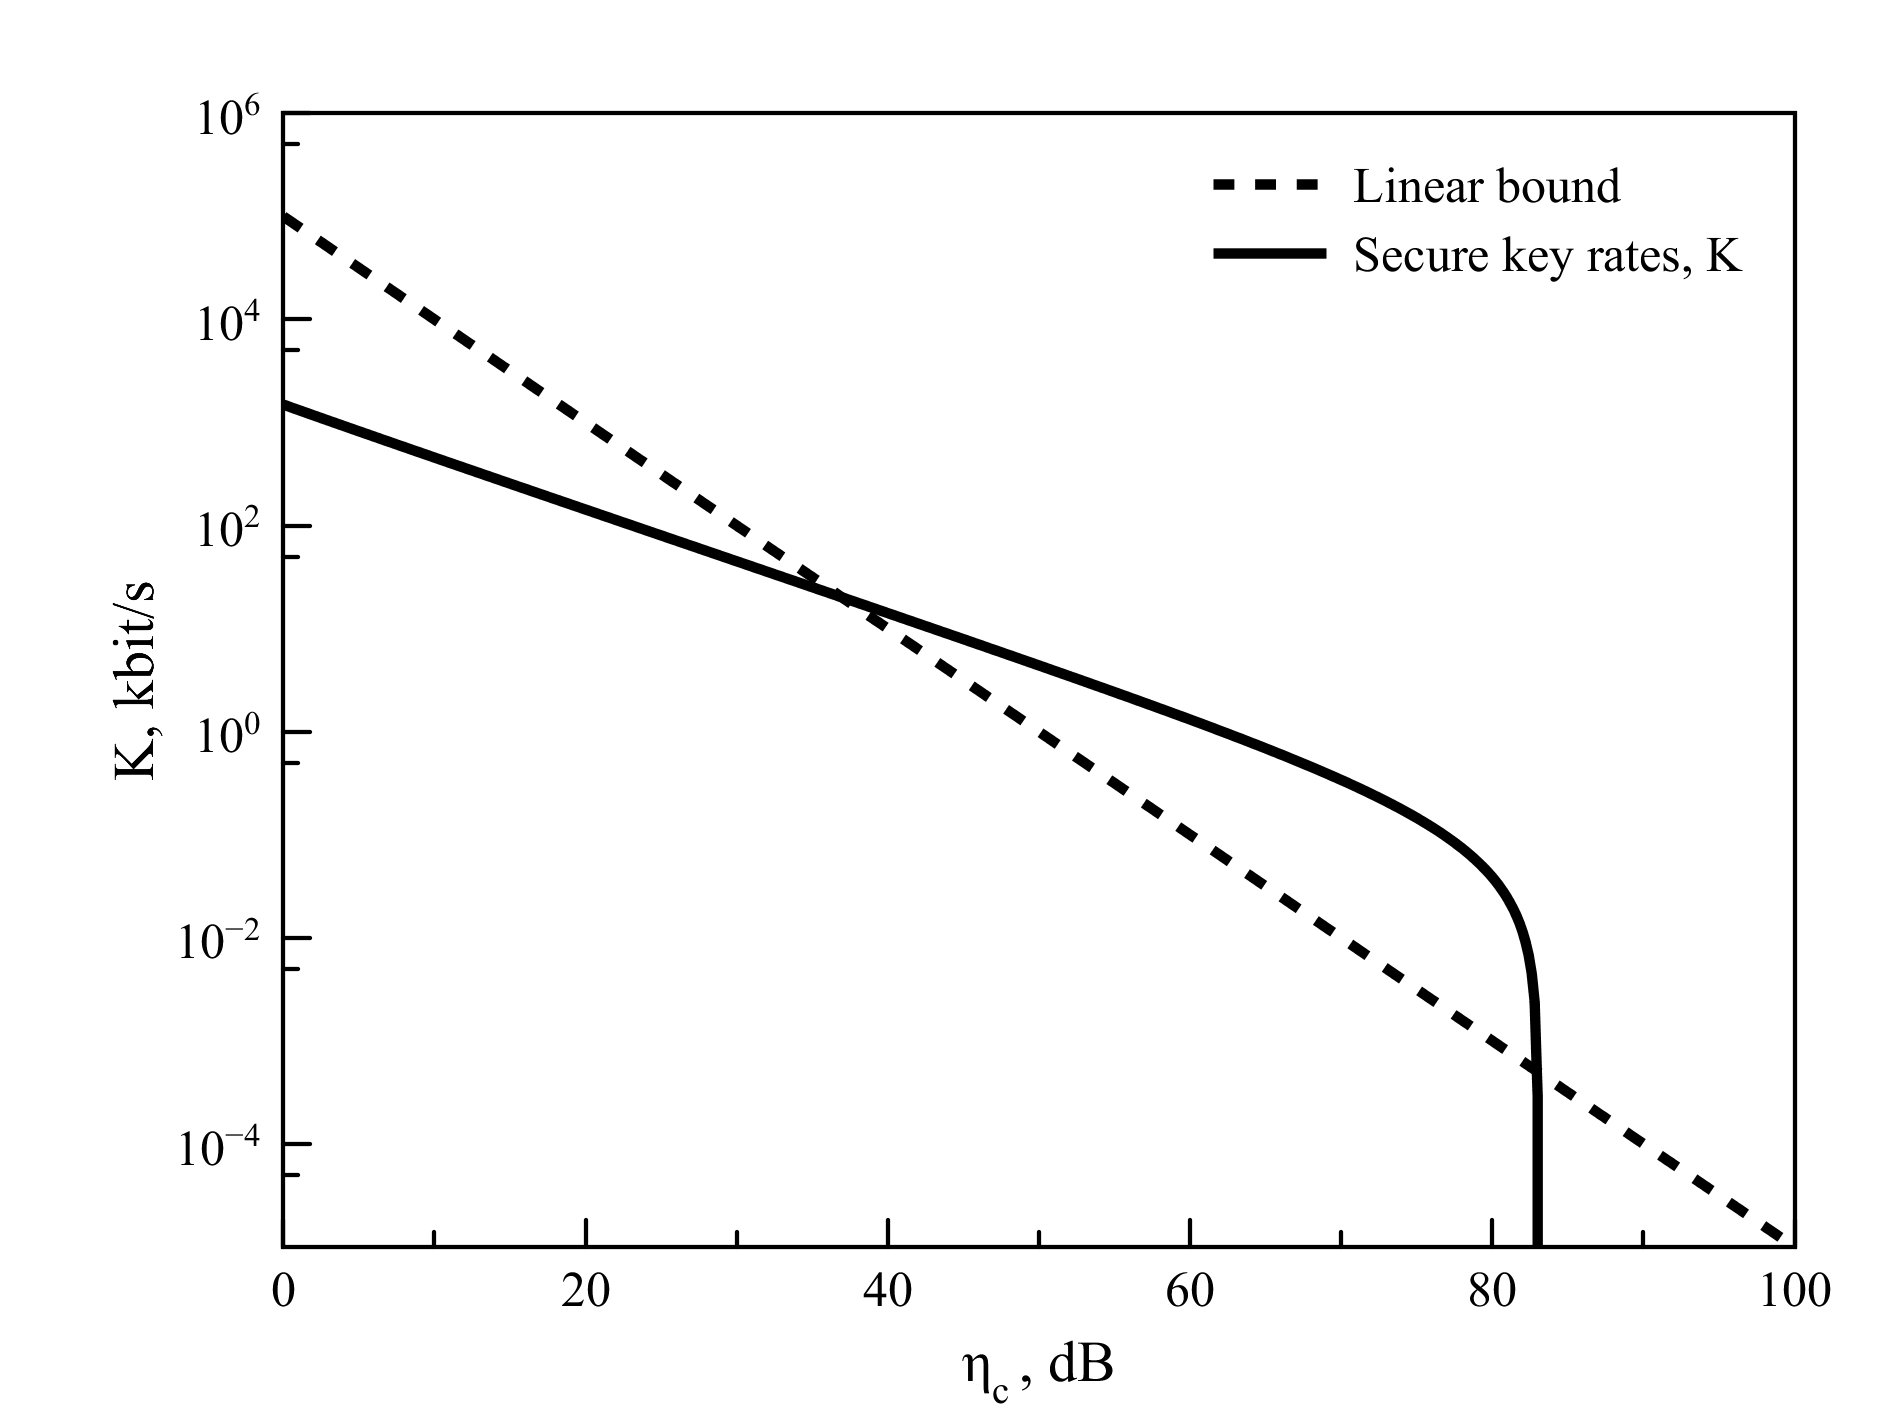
\includegraphics[width=1\linewidth]{TFQKD.png}
	\caption{ Simulation of our TF QKD protocol based on multi-mode phase-coded weak coherent states. For the considered simulation parameters, the key rate of proposed TF QKD exceeds the linear key rate bound by Pirandola et al. (PLOB bound) \cite{pirandola2017fundamental} when $\eta_c \gtrsim$ 40 dB (200 km). In addition, our protocol is also able to achieve a long transmission distance of $\eta_c\approx$ 83 dB (460 km). %Parameters were estimated as follows: $\mu=0.2$, $\mu_0=4$, $F=100$ MHz, $\gamma_{dark}=1.5$ kHz, $\vartheta=10^{-2.5}$, $\varphi_0\approx0$, $\eta=10^{-1.65}$, $\varphi_m\approx3^{\circ}$.} 
	}
	\label{fig:fig2}
\end{figure}


Наконец, можно определить выражение для оценки среднего значения скорости формирования просеянного ключа $K$ (одинаковые биты между легитимными пользователями, но коррелирующие с возможным результатом у злоумышленника, что требует проведения процедуры усиления секретности)
\begin{equation}
    K=FR(1-h(Q)),
\end{equation}
где $h(Q)$ это функция двоичной энтропии. 

\pagebreak

%%%%%%%%%%%%%%%%%%%%%%%%%%%%%%%%%%%%%%%%%%%%%%%%%%%%%%%%%%%%%%%%%%%%%%%%%%%%%%%%%%
\section{Выводы по главе} \label{ch:ch6/sec9}


В \ref{ch:ch6/sec2}  

\pagebreak

